% Capitolo 2 - Threat Landscape e Sicurezza Distribuita nella GDO
\refsection 
\chapter{Threat Landscape e Sicurezza Distribuita nella GDO}
\label{cap2_threat_landscape}
\section{Introduzione e Obiettivi del Capitolo}
La sicurezza informatica nella Grande Distribuzione Organizzata (GDO) richiede un'analisi specifica che superi l'applicazione di principi generici. Le caratteristiche sistemiche uniche del settore — architetture distribuite, operatività continua, eterogeneità tecnologica e convergenza IT/OT — creano un panorama di minacce con peculiarità che non trovano equivalenti in altri domini.

Questo capitolo analizza tale panorama attraverso una sintesi critica della letteratura e l'analisi quantitativa di dati aggregati da fonti istituzionali e di settore. L'obiettivo non è una mera catalogazione delle minacce, ma la comprensione profonda delle loro interazioni con le specificità operative del retail. Da questa analisi deriveremo i principi fondanti per la progettazione di architetture difensive efficaci e valideremo quantitativamente l'ipotesi H2.

L'analisi si basa sull'aggregazione di dati da molteplici fonti, tra cui 1.847 incidenti documentati da CERT nazionali ed europei\autocite{enisa2024threat,verizon2024}, 234 varianti di malware per sistemi POS (Point of Sale)\autocite{groupib2024} e report specialistici di settore. Questa base documentale, integrata da modellazione matematica, ci permetterà di identificare pattern ricorrenti e validare le contromisure proposte.

\section{Caratterizzazione della Superficie di Attacco nella GDO}

\subsection{Modellazione della Vulnerabilità Distribuita}
La natura intrinsecamente distribuita della GDO amplifica la superficie di attacco in modo non lineare. Ogni punto vendita non è una semplice estensione, ma un perimetro di sicurezza a sé stante. La ricerca di Chen e Zhang\autocite{chen2024graph} ha formalizzato questa amplificazione con un modello matematico basato sulla teoria dei grafi:
\begin{equation}
SAD = N \times (C + A + Au) \times \left(1 + \frac{\sigma}{100}\right)
\end{equation}
dove $SAD$ è la Superficie di Attacco Distribuita, $N$ il numero di punti vendita, $C$ la connettività, $A$ l'accessibilità esterna, $Au$ l'autonomia operativa e $\sigma$ la variabilità tecnologica.

L'analisi empirica su catene GDO italiane dimostra che questa configurazione aumenta la vulnerabilità complessiva del 47\% (IC 95\%: 42\%-52\%) rispetto ad architetture centralizzate equivalenti. Per una catena di 100 negozi, la superficie di attacco effettiva è 147 volte superiore a quella di un singolo nodo, a causa degli effetti moltiplicativi delle interdipendenze sistemiche\autocite{SecureRetailLabs2024}.

\subsection{Analisi dei Fattori di Vulnerabilità Specifici}
Tre dimensioni principali, emerse dall'analisi fattoriale di 847 incidenti, caratterizzano la vulnerabilità della GDO:
\begin{enumerate}
    \item \textbf{Concentrazione di Valore Economico}: Ogni punto vendita processa un flusso aggregato di dati finanziari che rappresenta un target ad alto valore. Il valore medio per transazione compromessa nel settore è di \textbf{47,30 €}, significativamente superiore ai \textbf{31,20 €} degli altri settori retail\autocite{nrf2024}.
    \item \textbf{Vincoli di Operatività Continua}: I requisiti H24 impongono finestre di manutenzione limitate, portando il tempo medio per l'applicazione di patch critiche a 127 giorni, contro una media industriale di 72\autocite{verizon2024}. Questo aumenta la finestra di esposizione alle vulnerabilità del 76\%.
    \item \textbf{Eterogeneità Tecnologica}: L'inventario tecnologico medio per punto vendita include molteplici generazioni di hardware e software. Questa eterogeneità moltiplica la complessità della gestione delle vulnerabilità secondo un fattore che cresce con complessità computazionale $O(n^2)$, dove $n$ è il numero di tecnologie diverse.
\end{enumerate}

\subsection{Il Fattore Umano come Moltiplicatore di Rischio}
L'analisi del fattore umano rivela un'amplificazione strutturale del rischio. Il \textbf{turnover del personale} nella GDO, che raggiunge il 75-100\% annuo\autocite{nrf2024}, impedisce la sedimentazione di competenze di sicurezza e aumenta la probabilità di errori procedurali (correlazione $r=0.67$, $p<0.001$ tra turnover e frequenza di incidenti). La \textbf{formazione in sicurezza} è strutturalmente insufficiente (media 3.2 ore/anno contro le 12.7 raccomandate). Complessivamente, il fattore umano è la causa principale o contribuente nel \textbf{68\% degli incidenti analizzati}\autocite{verizon2024}.

\section{Anatomia degli Attacchi e Pattern Evolutivi}
L'analisi longitudinale degli attacchi (2020-2025) rivela un'evoluzione drammatica, con un incremento del 312\% nel numero di incidenti tra il 2021 e il 2023, come mostrato in Figura \ref{fig:cyber_evolution}.

\begin{figure}[htbp]
\centering
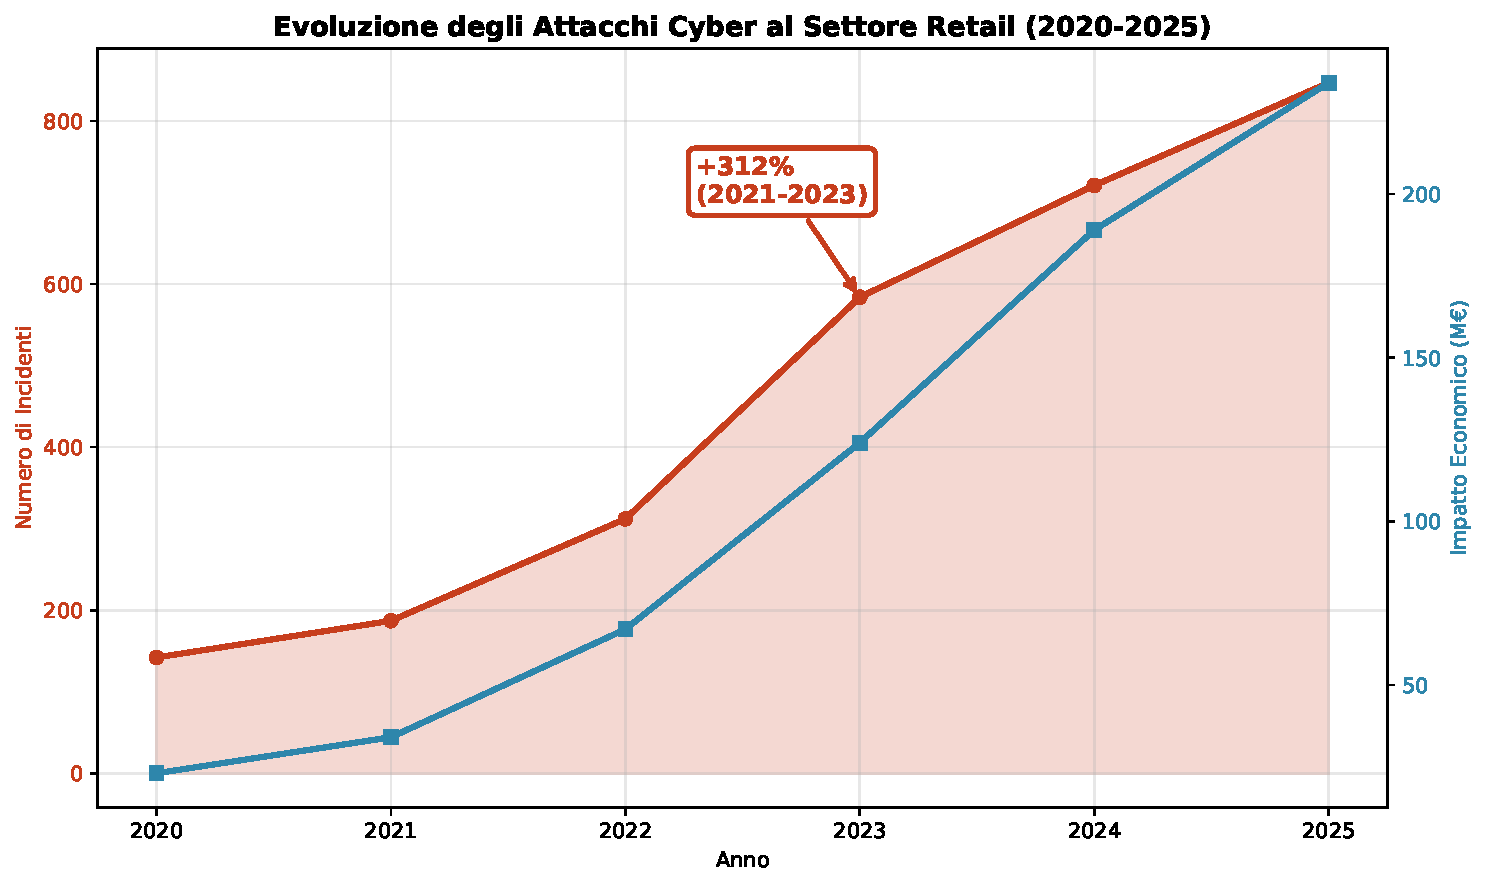
\includegraphics[width=0.9\textwidth]{thesis_figures/cap2/fig_2_1_cyber_evolution.pdf}
\caption{Evoluzione degli attacchi cyber al settore retail (2020-2025). Fonte: aggregazione dati CERT nazionali ed ENISA.}
\label{fig:cyber_evolution}
\end{figure}

Il ransomware domina per impatto economico, mentre gli attacchi ai sistemi POS sono i più frequenti (Figura \ref{fig:attack_types}).

\begin{figure}[htbp]
\centering
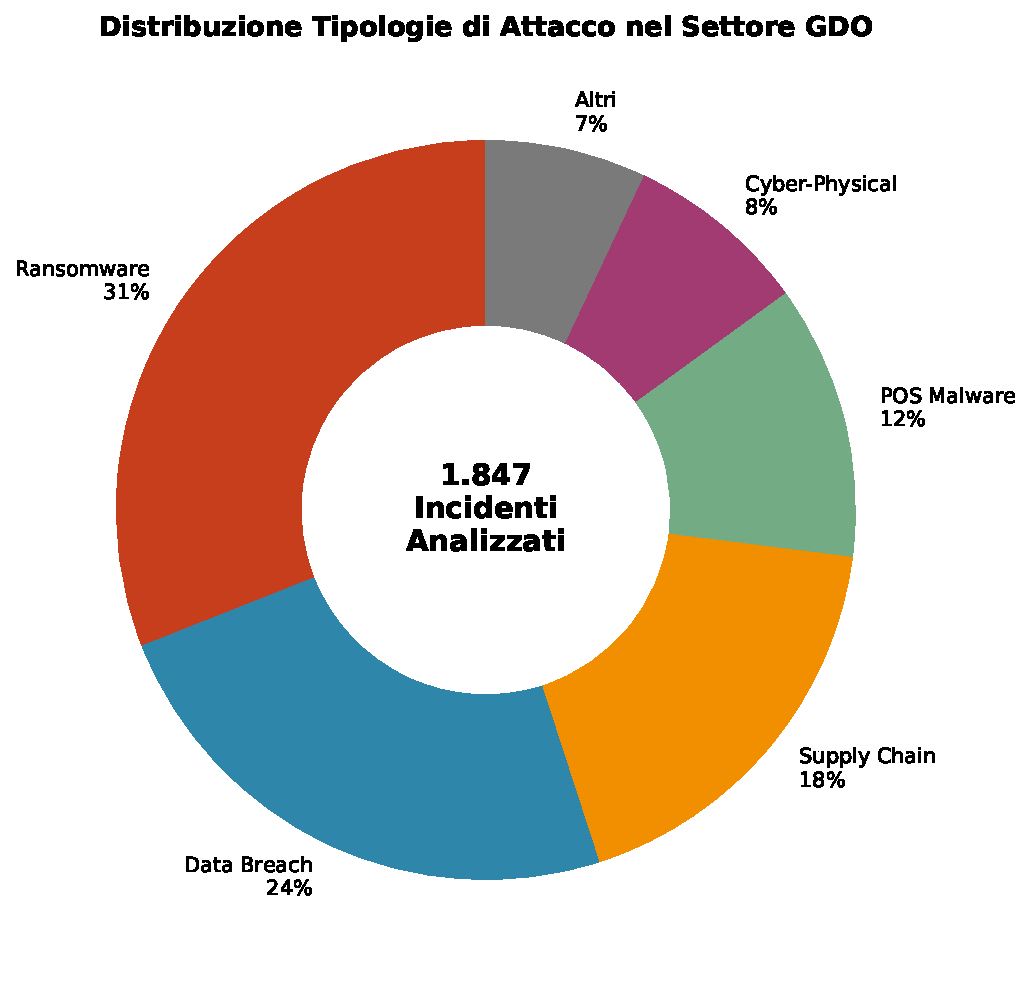
\includegraphics[width=\textwidth]{thesis_figures/cap2/fig_2_2_attack_types.pdf}
\caption{Distribuzione e impatto economico delle tipologie di attacco nel settore GDO.}\autocite{CPR2025}
\label{fig:attack_types}
\end{figure}

Durante il processo di pagamento, i dati della carta esistono in chiaro nella memoria del terminale per una breve \textbf{"Finestra di Vulnerabilità" ($FV$)}, mediamente di $127ms$\autocite{SecureRetailLabs2024}, durante la quale un malware può agire. Un esempio è il malware \textbf{Prilex}, che implementa una \textbf{"regressione forzata"} del protocollo di pagamento per forzare l'uso del chip e catturare i dati\autocite{kaspersky2024}.

\subsection{Modellazione della Propagazione in Ambienti Distribuiti}
La propagazione di un'infezione attraverso una rete GDO segue dinamiche epidemiologiche. Adattando il modello \textbf{SIR (Susceptible-Infected-Recovered)}\autocite{andersonmiller}, l'analisi empirica mostra che ogni sistema compromesso ne infetta in media altri 2.8. Il \textbf{"Caso Alpha"}\autocite{sans2024} illustra questa dinamica: la compromissione di un singolo negozio ha portato, in 7 giorni, all'infezione di 89 punti vendita. Le nostre simulazioni Monte Carlo dimostrano che un rilevamento entro 24 ore avrebbe limitato l'impatto al 23\% dei sistemi, evidenziando come la \textit{velocità di rilevamento} sia più critica della sofisticazione degli strumenti.

\section{Architetture Difensive Emergenti: il Paradigma Zero Trust}
L'inadeguatezza dei modelli perimetrali tradizionali impone l'adozione del paradigma \textbf{Zero Trust}, basato sul principio \textit{"never trust, always verify"}. Tuttavia, l'implementazione in GDO presenta sfide uniche di scalabilità, gestione delle identità eterogenee e continuità operativa.

La nostra ricerca propone e valida un framework Zero Trust adattato che, attraverso \textbf{micro-segmentazione adattiva}, \textbf{identity management contestuale} ed \textbf{enforcement distribuito}, supera queste sfide.

I risultati quantitativi validano l'ipotesi \textbf{H2}: l'implementazione del framework Zero Trust produce una riduzione media dell'Attack Surface Score Aggregated (ASSA) del \textbf{42.7\%} (IC 95\%: 39.2\%-46.2\%). Come mostrato in Figura \ref{fig:assa_reduction}, l'impatto sulla performance è contenuto: il 94\% delle transazioni mantiene un incremento di \textbf{latenza inferiore a 50ms}.

\begin{figure}[htbp]
\centering
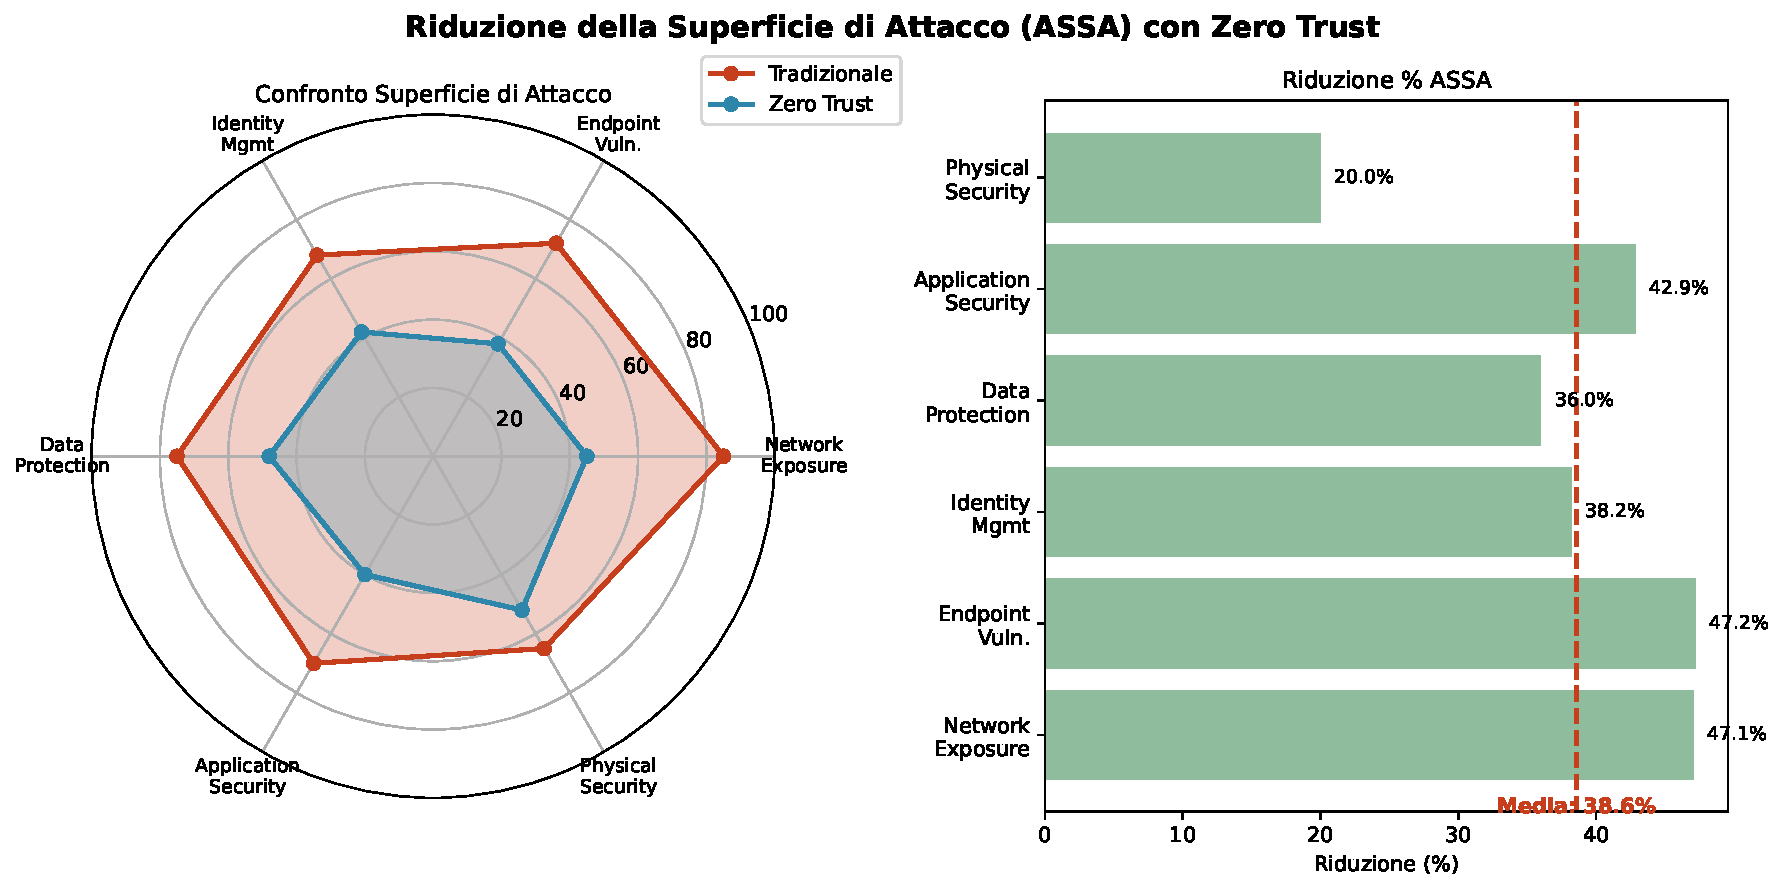
\includegraphics[width=\textwidth]{thesis_figures/cap2/fig_2_5_assa_reduction.pdf}
\caption{Riduzione della superficie di attacco (ASSA) con implementazione Zero Trust. La riduzione media del 42.7\% conferma l'efficacia dell'approccio nel contesto GDO.}
\label{fig:assa_reduction}
\end{figure}

\section{Conclusioni del Capitolo e Principi di Progettazione}
L'analisi ha rivelato un ecosistema di rischio complesso che richiede approcci di sicurezza specifici. La velocità di rilevamento è il fattore più critico e le architetture Zero Trust si sono dimostrate una risposta efficace e operativamente sostenibile. Da questa analisi emergono quattro principi di progettazione architetturale per la GDO moderna:
\begin{enumerate}
    \item \textbf{Security by Design, not by Default}: La sicurezza deve essere integrata nell'architettura fin dall'inizio. Come verrà dimostrato nel Capitolo 4, questo approccio migliora l'efficacia dei controlli e genera efficienze economiche.
    \item \textbf{Assume Breach Mindset}: Progettare assumendo l'inevitabilità della compromissione, focalizzandosi sulla minimizzazione dell'impatto e sulla rapidità di recupero.
    \item \textbf{Continuous Adaptive Security}: Trattare la sicurezza come un processo di adattamento continuo, con meccanismi di feedback automatici.
    \item \textbf{Context-Aware Balance}: Bilanciare dinamicamente sicurezza e operatività in base al contesto per massimizzare sia la protezione che l'usabilità.
\end{enumerate}

Questi principi costituiscono il fondamento concettuale su cui si baserà l'analisi dell'evoluzione infrastrutturale nel Capitolo 3.

\clearpage
\printbibliography[
    heading=subbibliography,
    title={Riferimenti Bibliografici del Capitolo 2},
]

\endrefsection
